The testing implementation was developed with high modularity in
mind, since it is meant to be a proof-of-concept implementation and
not a a production grade system. High modularity also makes
development easier and the system more robust against changes, two
very important qualities during this project.

The implementation is written in Python and consists of three main parts:
\begin{description}
  \item[Particle Filter] A direct  implementation of the procedure in
    table \ref{alg:pf}.
  \item[Database] A database with functions for extracting transition
    hypotheses. Provides the prediction PDF $\cprobnext{x}$ to the
    particle filter.
  \item[Tracker] Manages the model and performs matching between
    hypotheses and images. Provides the filtering PDF
    $\cprob{I_n}{x_n}$ to the particle filter.
\end{description}

\section{The particle filter}

The particle filter implementation is a direct implementation of the
procedure in table \ref{alg:pf}. It is implemented as a function that
takes the parameters $X_{t-1}$, $I_t$, \texttt{importance\_function} and
\texttt{sampling\_function}. The parameters are the hypotheses from
the last time step, the current video frame and the functions to use
as \textsc{Predict} and \textsc{Importance} in \ref{alg:pf},
respectively. This means that the particle filter function is general
and independent of the model used.

\subsection{Initilization $x_0$}
The test implementation needs to be manually initialized. When
tracking generated whiskers, the states were always known and program
could therefore be programmatically inserted. When testing on real
whiskers, the start states were calculated by manually
selecting pixels along each whisker and using a MATLAB script to find
the least squares solution for the coefficients $\langle a_1, a_2, a_3 \rangle$.

\subsection{Prediction $\cprobnext{x}$}
The \textsc{Predict} function was implemented as a weighted mean of the
state transitions in the database. The function is stated in table
\ref{alg:predict}. Notice the parameters $a$ and $p$. $p$ is a
positive integer that determines which $\Lp$ space to compute the norm
in. $a$ is a positive number, and determines how fast the weight $w$
declines with the distance $\Lpnorm[p]{\tf - x_{t-1}}$, see figure
\ref{fig:x-to-the-minus-a}. A high $a$ means closer transitions get a
much higher weight than ones far away.

\begin{figure}
  \centering
  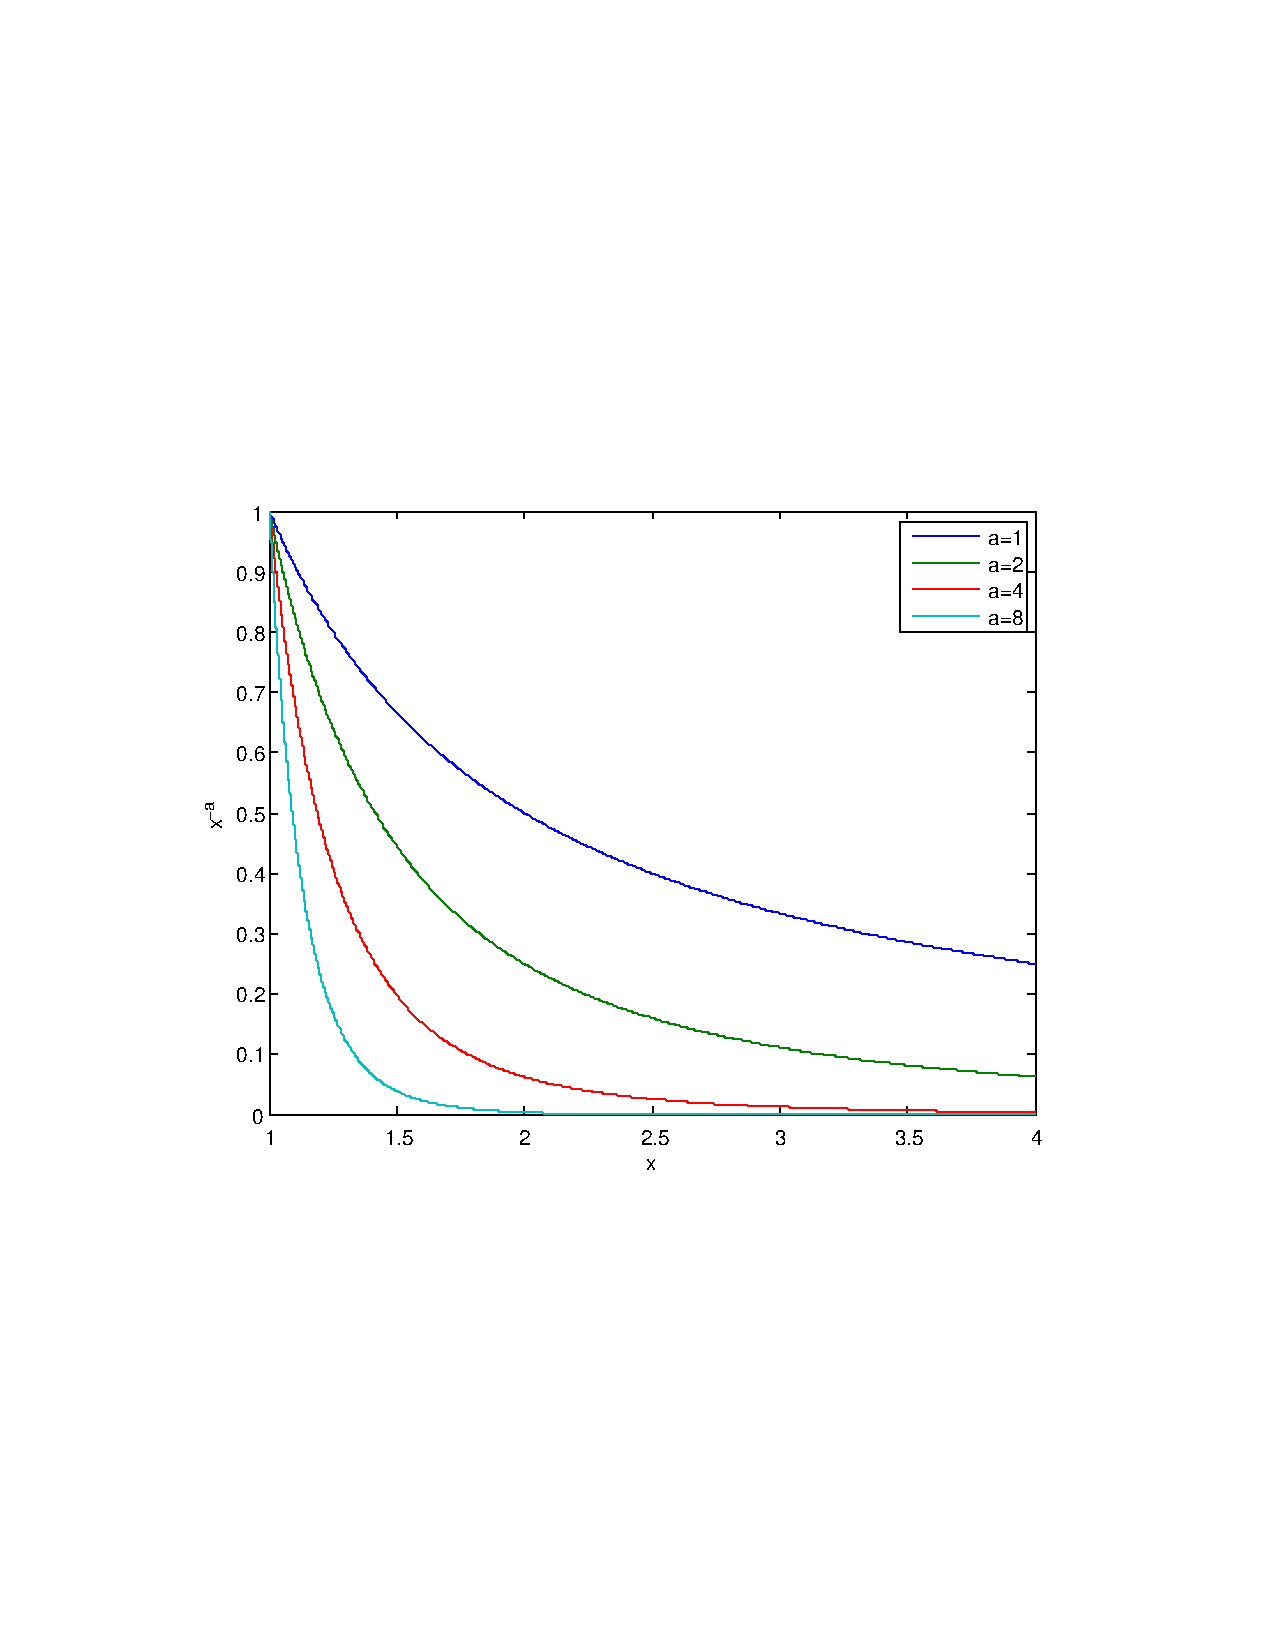
\includegraphics[width=0.8\textwidth,trim=20mm 20mm 20mm 20mm]{x-to-the-minus-a.pdf}
  \caption{$x^{-a}$ versus $x$. TODO: Crop it!}
  \label{fig:x-to-the-minus-a}
\end{figure}

\begin{table}
  \begin{codebox}
    \Procname{$\proc{Predict} (x_{t-1})$}
    \li $ x_{t-1} \gets 0$
    \li $ W \gets 0$
    \li \ForEach $(\tf, \tt) \in \proc{Database-Get-All}()$
    \li \Do
      \li $ w \gets \left(\Lpnorm[p]{\tf - x_t}\right)^{-a}$
      \li $ x_t \gets x_t + \tt$
      \li $ W \gets W + w$
    \End
    \li \Return $x_t / W$
  \end{codebox}
  \caption{The prediction function, with the parameters $a$ and $p$.}
  \label{alg:predict}
\end{table}



\subsection{Goodness $\kappa\cprob{x_t}{I_t}$}
It also needs an direction to know how good the hypothesis $x_t$ matches the given image $I_t$.

TODO <ref:theorem>

...

\section{The state transition database}





\section{Real data}
    \subsection{Pre-processing}

    We want to find the function $\prob{I=\text{whisker}}\in\IS$

    >We want to have a measure on how probable it is for a pixel to hosehould a whisker





